\documentclass[a4paper,12pt]{article}
\usepackage{graphicx}
\usepackage{titling}

\setlength{\droptitle}{-14em}
\title{Is Florida getting warmer?}
\author{Zhongbin Hu}
\date{21/10/2023}

\begin{document}

  \maketitle

  \section{Results}
  \begin{figure}[h]
    \centering
    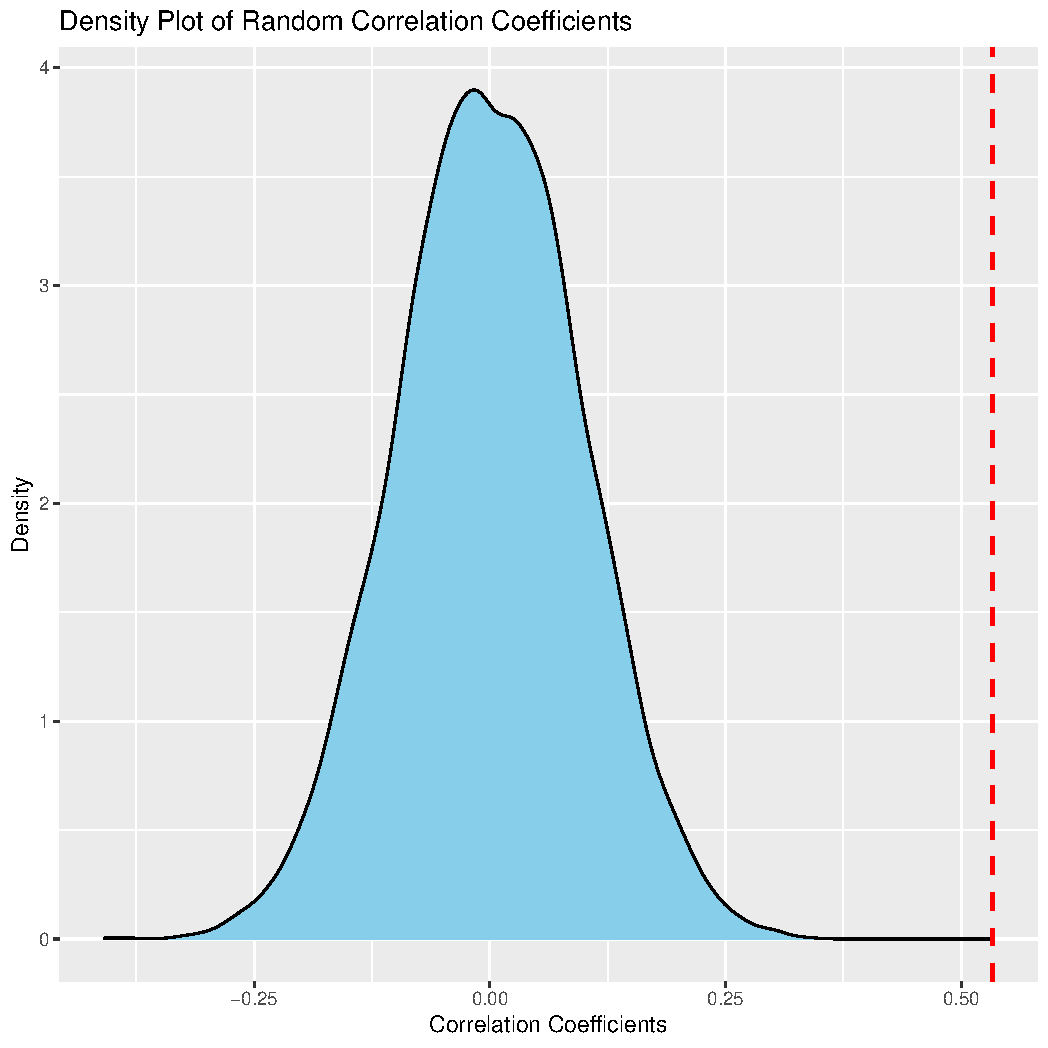
\includegraphics[width=0.7\textwidth]{../results/Florida_plot.pdf}
    \caption{Distribution of Permutation Correlation Coefficients with Observed Coefficient}
    \label{Florida}
  \end{figure}

The figure above includes the permuted corrlation coefficients and observed coefficient(red line).The observed correlation coefficient between years and temperature in the original dataset was calculated to be around 0.5331784. 
After 10,000 permutations and caculation, it was found that all of 10,000 permuted correlation coefficients were smaller or equal than the observed one. The approximate p-value is 0 after caculation.

\section{Interpretation}
From the figure the permuted correlation coefficients is nearly normaly distributed, and the observed coefficient is larger than all the permuted coefficient. This means the observed coefficient hardly occured by random chance.
In addition, the approximate samll p-value obtained from the permutation test suggests that the correlation between years and temperature is statistically significant.
Since the observed coefficient is larger than 0, there is a positive correlation between the year and temperature.
Therefore, the data supports the hypothesis that there is a significant correlation between the year and temperature Florida during the 20th century and Florida is becoming warmer.


\end{document}
